%DO NOT MESS AROUND WITH THE CODE ON THIS PAGE UNLESS YOU %REALLY KNOW WHAT YOU ARE DOING
\chapter{Experimental research} \label{Experimental research}

\noindent By using the formula for velocity of speed in ocean, the graph of velocity of speed in ocean versus depth is plotted for various values of temperature. 

\begin{figure}[H]
\centering
{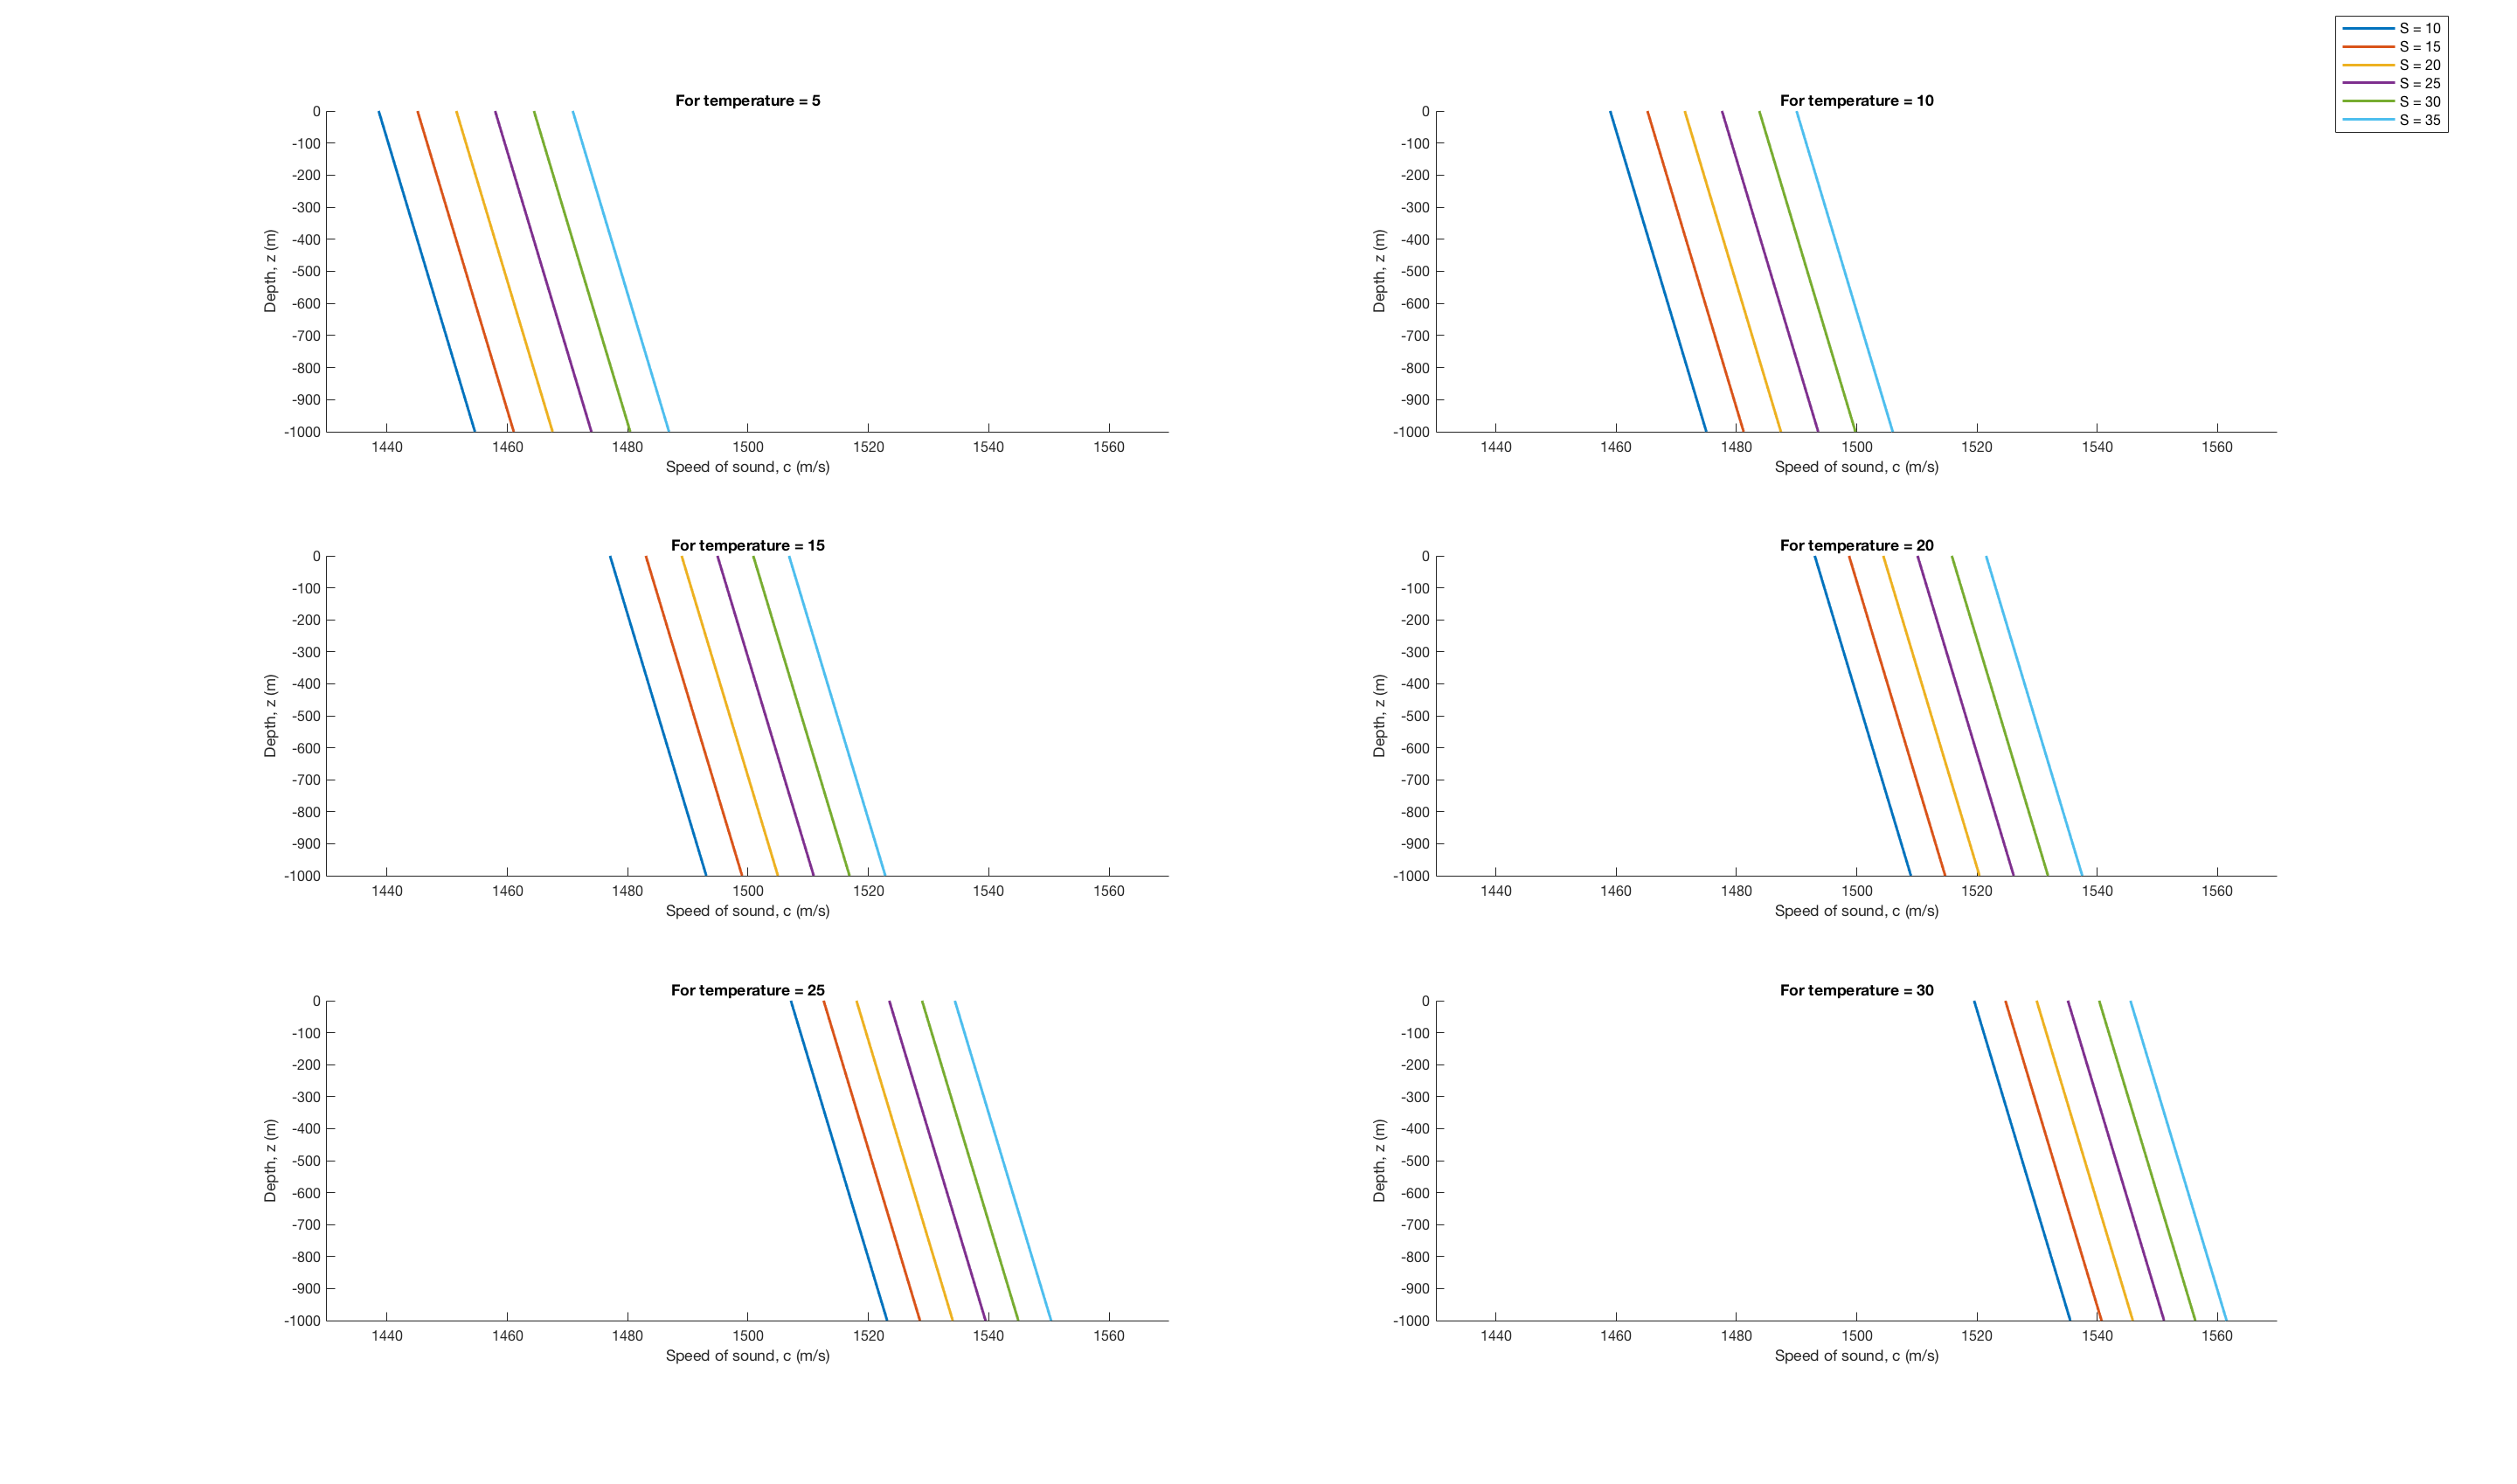
\includegraphics[scale=0.18]{ucp1.png}}
\caption{c versus z for various sets of T}
\end{figure}

\noindent By using the formula for velocity of speed in ocean, the graph of velocity of speed in ocean versus depth for various values of salinity is obtained. 

\begin{figure}[H]
\centering
{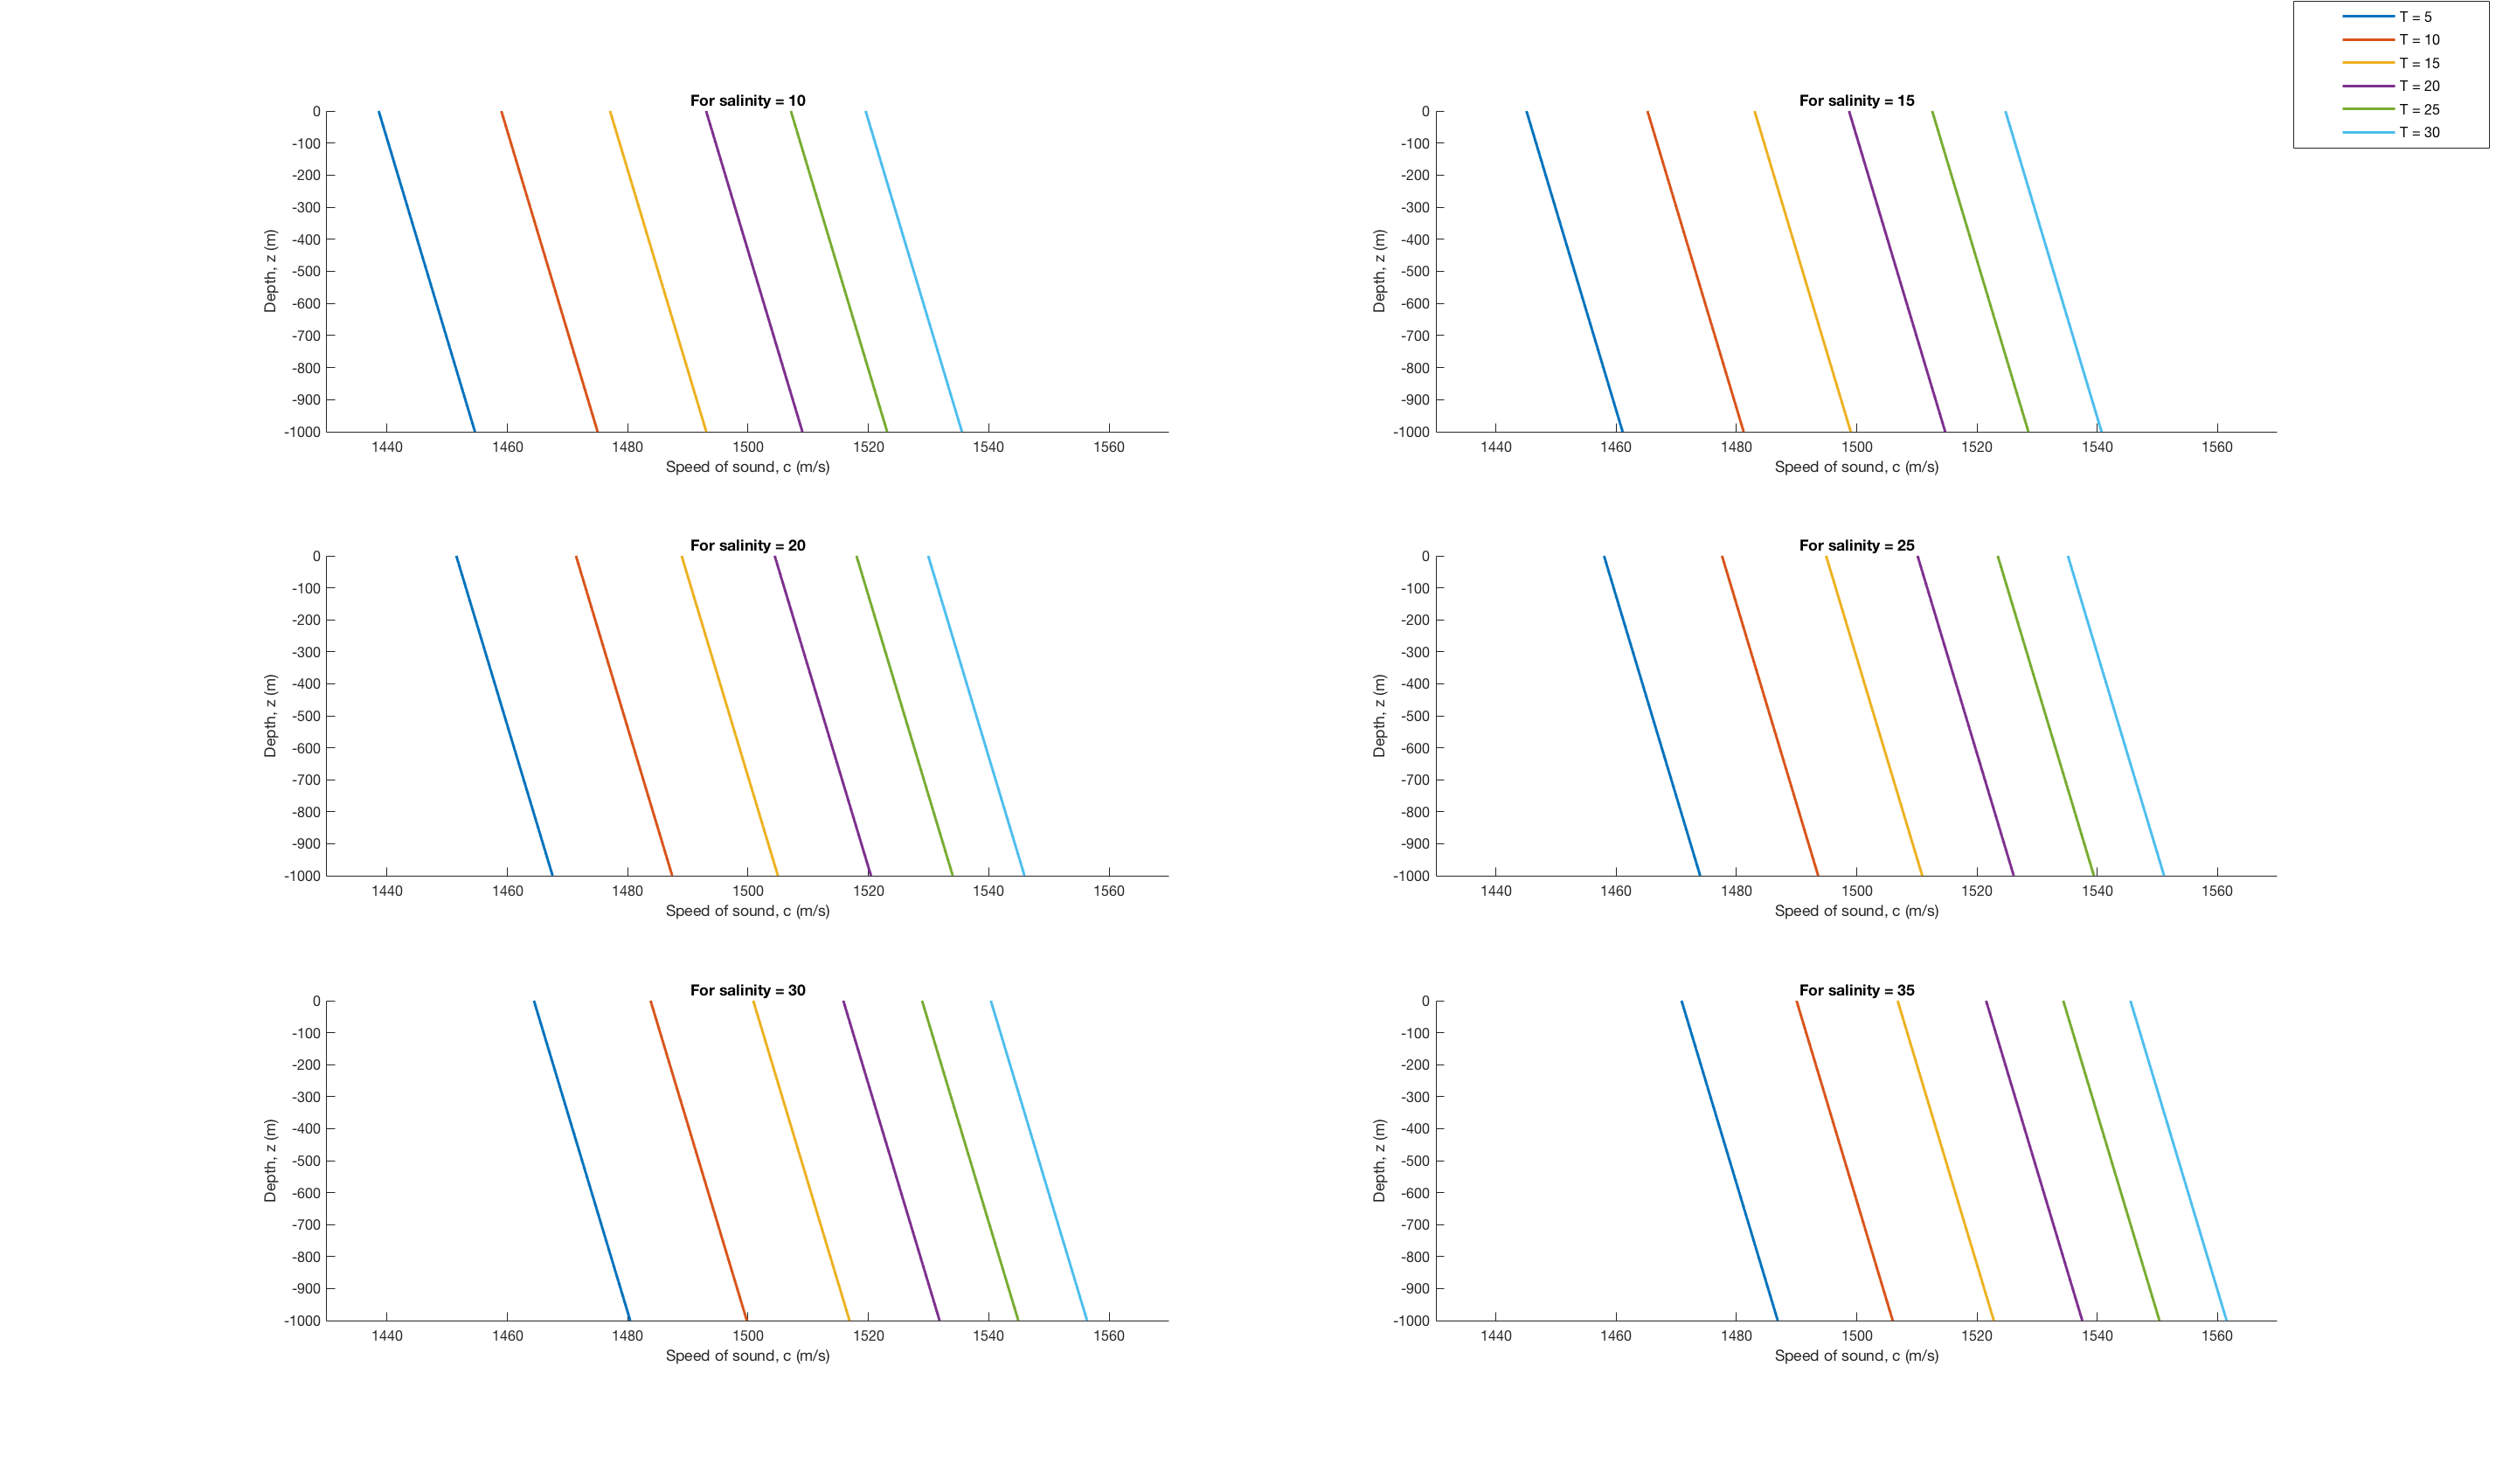
\includegraphics[scale=0.18]{ucp2.png}}
\caption{c versus z for various sets of S}
\end{figure}

\noindent The dependency of non-linear temperature profile and depth is plotted using an exponential function for temperature. The plot contains of three curves: temperature versus depth, sound velocity (having constant salinity and temperature) versus depth and sound velocity (having expoenential temperature and constant salinity) versus depth.

\begin{figure}[H]
\centering
{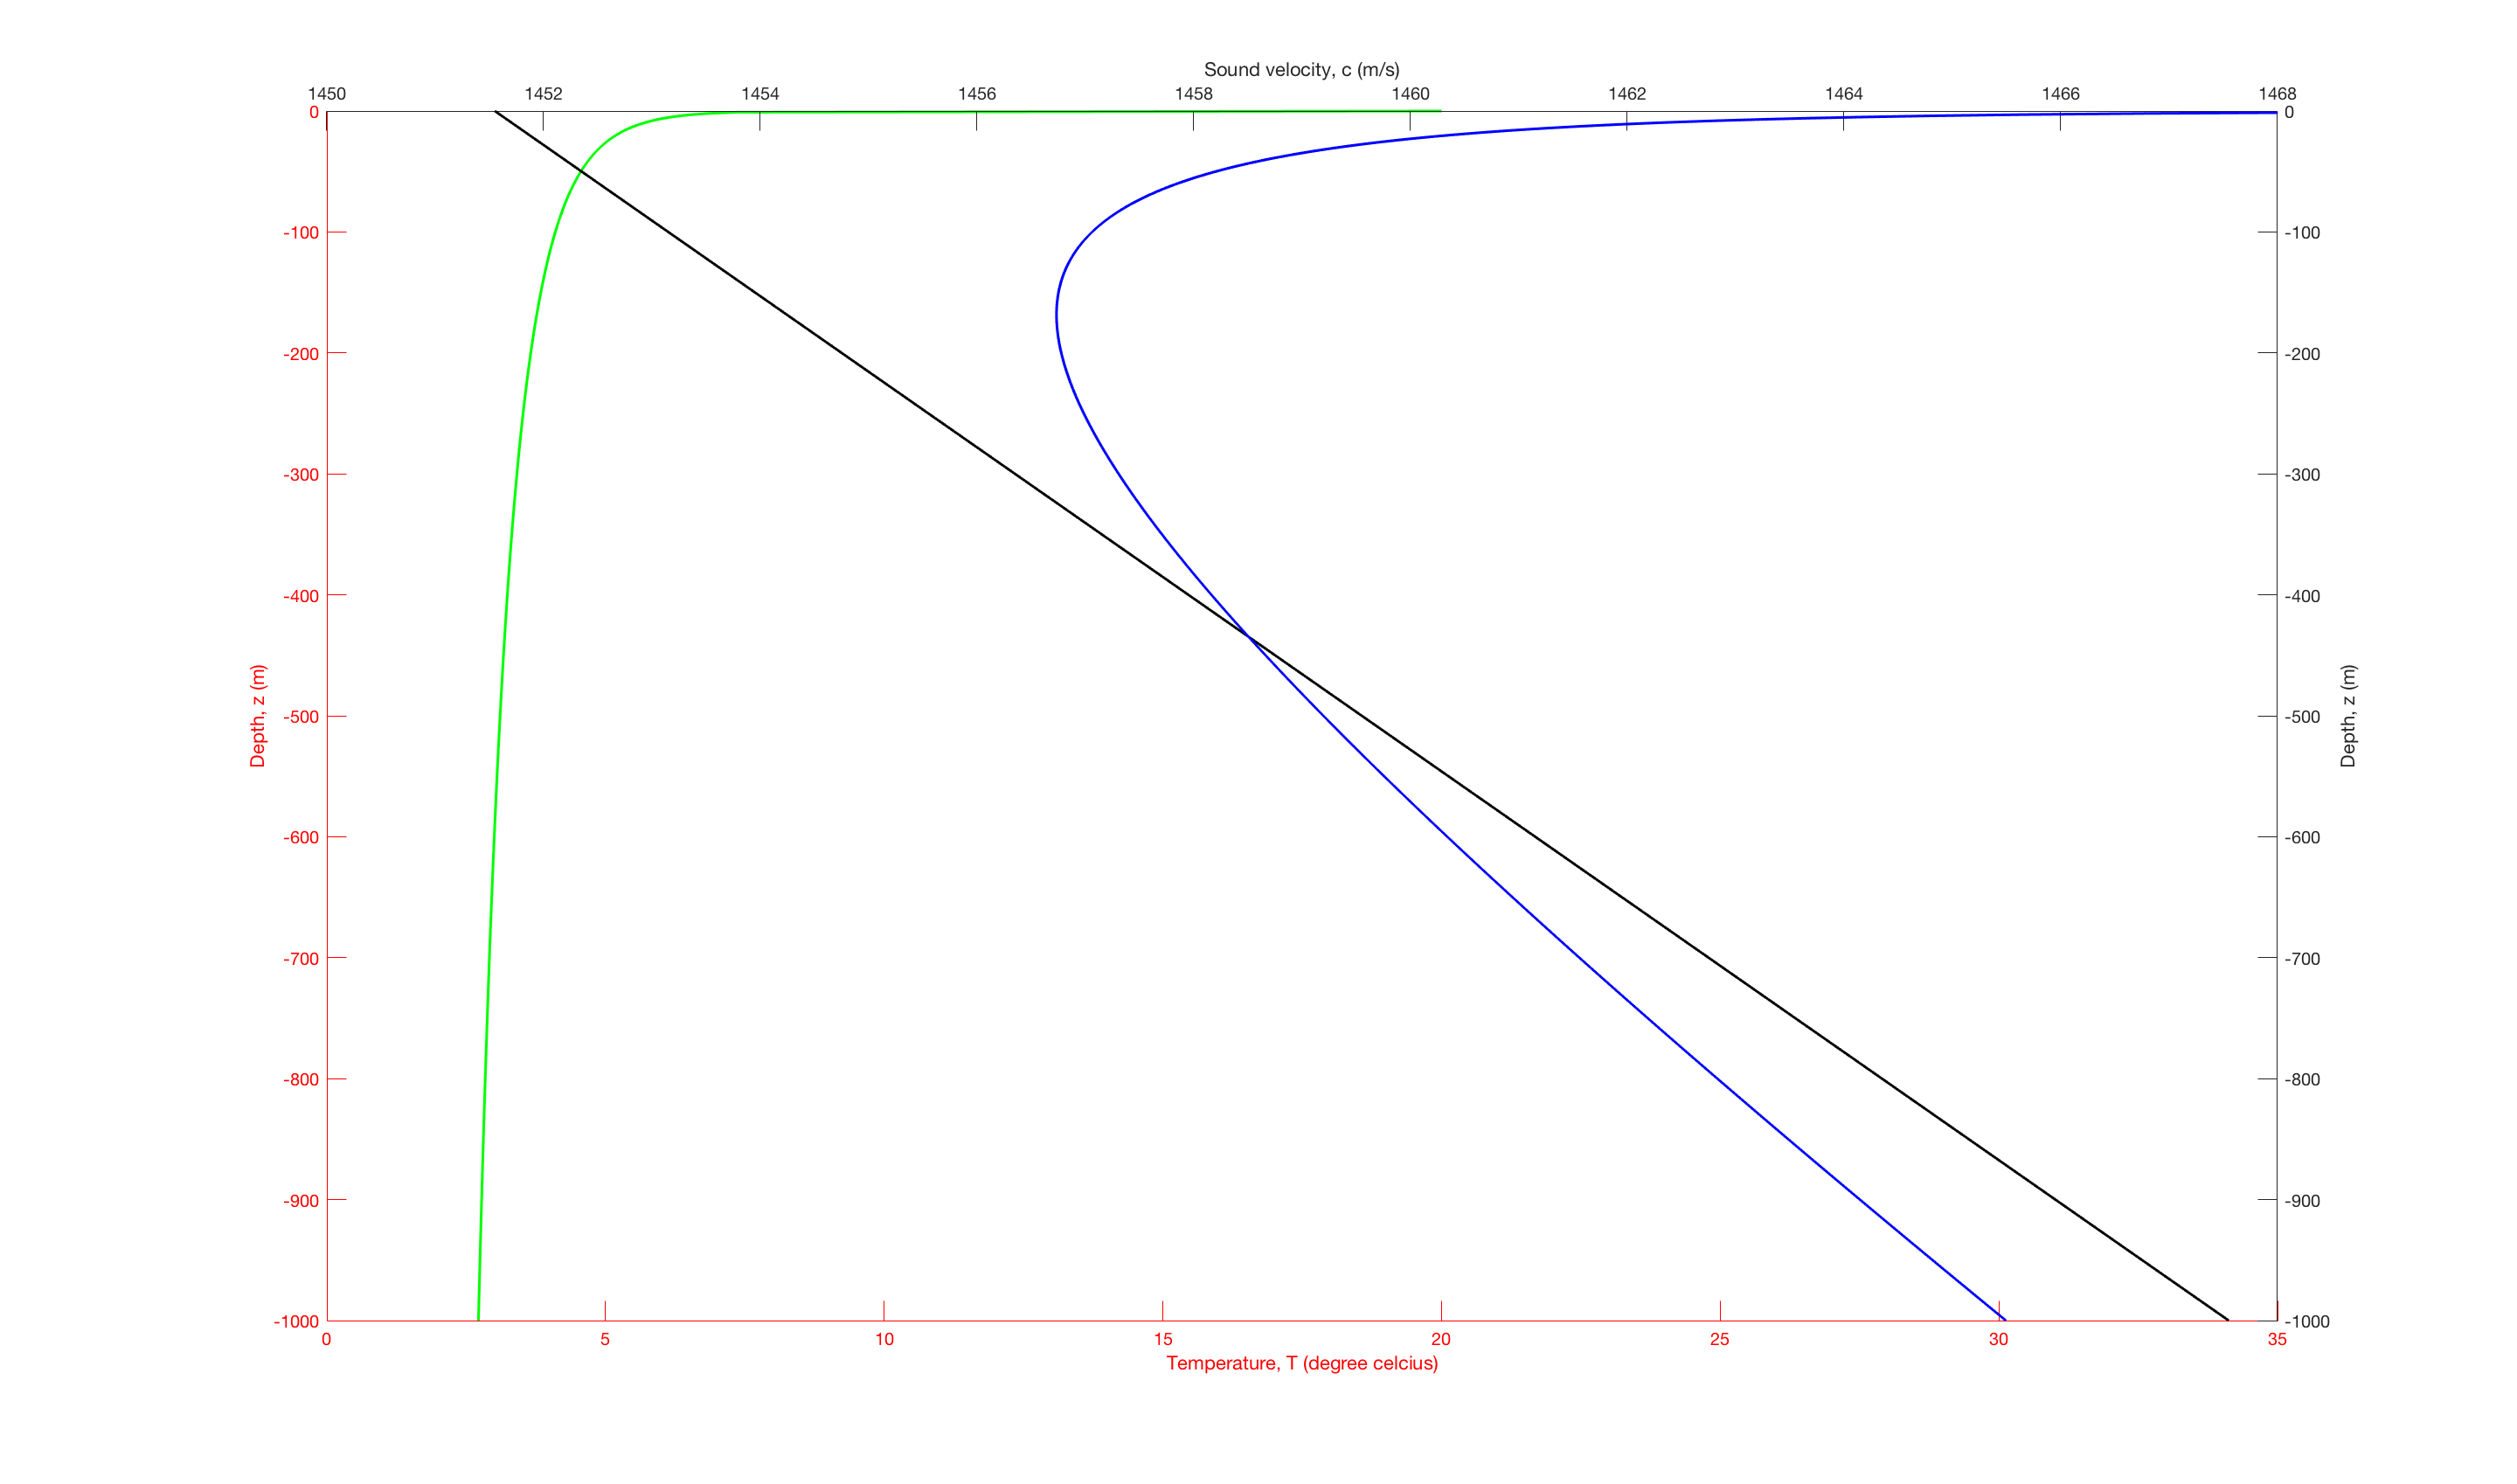
\includegraphics[scale=0.18]{nonlinear.png}}
\caption{Dependency of non-linear temperature profile and depth}
\end{figure}
